\documentclass[12pt]{article}
\usepackage[top=1in, bottom=1in, left=1in, right=1in]{geometry}
\usepackage[justification=centering]{caption}
\usepackage{graphicx}
\usepackage{listings}
\usepackage{color}
\usepackage{indentfirst}
\usepackage{hyperref}
\usepackage{siunitx}
\usepackage{float}
\usepackage{amsmath}

\lstset{ %
	%language=C,                % choose the language of the code
	basicstyle=\scriptsize,       % the size of the fonts that are used for the code
	                  % how far the line-numbers are from the code
	backgroundcolor=\color{white},  % choose the background color. You must add \usepackage{color}
	showspaces=false,               % show spaces adding particular underscores
	showstringspaces=false,         % underline spaces within strings
	showtabs=false,                 % show tabs within strings adding particular underscores
	%frame=single,           % adds a frame around the code
	tabsize=2,          % sets default tabsize to 2 spaces
	captionpos=b,           % sets the caption-position to bottom
	breaklines=true,        % sets automatic line breaking
	breakatwhitespace=false,    % sets if automatic breaks should only happen at whitespace
	escapeinside={\%*}{*)}          % if you want to add a comment within your code
}

\begin{document}
\title{Microprocessor Systems\\ Lab 5: Memory Interfacing }
\author{Nick Choi \and Samuel Deslandes}
\date{11/14/16}
\maketitle
\pagebreak
\section{Introduction}


\section{Methods}
\subsection{Software}
The code for parts 1, 2 and 3 can be found in Appendix A, B and C respectively. All code was uploaded and run on the 8051 through the programming/debugging USB port. 

\subsubsection{Part 1}
In the first section of the lab, a C program was written to write a value to address \texttt{0x1FF0}, an on-board address space on the 8051. This address is then read and its value written to all of the addresses on the Am9128: \texttt{0x2000}--\texttt{0x27FF}. Each time a value was written it was immediately read back and printed to the terminal to ensure the chip was performing properly and that the value read was the same as what was written. Address \texttt{0x2800}, beyond the range of the 2k chip, was also written to, with the expectation that no value would be read back.

In order to interface with the memory chips, the EMI0CF SFR must be configured such that ports 4--7 are used as data buses, address buses, or control signals for the chip, and that EMIF operates in split mode with bank select. This can be done by setting EMI0CF to \texttt{0x3B}. The EMI0TC SFR is used for timing control for the chips. Since these are older chips, the slowest setting are used, which is done by setting EMI0TC to \texttt{0xFF}. In addition to this, ports 4--7 were configured for push-pull operation using the PnMDOUT SFRs. 

In order to access certain memory addresses pointers declared with the ``\_\_xdata'' keyword were used. The program starts by initializing a pointer to address \texttt{0x1FF0} and writing the character `a' to it. This address is then read and printed to the terminal in order to verify the character `a' gets read back. The pointer is then changed to point to address \texttt{0x2000}, and using a loop the value previously read is written the pointer\textquoteright s location, with the pointer being incremented at the end of the loop. As described above, the loop terminates at address \texttt{0x2800}, at which point the dereferenced pointer cannot be read.

\subsubsection{Part 2}
In principle the program for this part is the same as that of part 1, the main difference being the address range used is now \texttt{0x2800}--\texttt{0x2FFF}. This program writes `\texttt{0xAA}' to all of the addresses in this range, immediately reading them back and printing the result to the terminal. This process is then repeated using the value `\texttt{0x55}'. To ensure that all addresses are being updated accordingly, any addresses that do not read back the expected `\texttt{0x55}' are added to an array. At the end of the program the contents of this array are printed to the terminal.

\subsubsection{Part 3}
The program for this part is meant for interfacing with the Am91L14 1024x4 chip, starting at address \texttt{0x4000}. First, an array is initialized with the values 0--15. Values will be written from this array to the memory on the Am91L14. This is accomplished using pointers and the same methods described in part 1. 

\subsubsection{Enchancement}
An enhancement was made to the program described in part 1. This program queries the user for a starting address (within the range \texttt{0x1FF0}--\texttt{0x1FFF}), and a 4-bit value used for writing to address spaces. Once the input has been parsed, the program writes the value to all of the additional external spaces, reading back the result to the terminal. This represented the range \texttt{0x2000}--\texttt{0x4400}, with the values in the range of \texttt{0x3000}--\texttt{0x3FFF} reading back garbage data as none of the chips were enabled in this range. 

In order to parse the user input from character inputs to hex values, the program first had to check whether the input was a digit. This was done using the built-in C function `isdigit()'. If the input was a digit, subtracting 48 (ASCII for `0') would result in the appropriate value (0--9). If the input was not a digit, the program would then check that the input is in the range of letters used by the hexadecimal number system (`A'--`F') and used a similar subtraction method to get the appropriate value. In the case of a capital letter input, 55 was subtracted (ASCII for `7'), and if the input was lowercase 87 was subtracted (ASCII for `W').

Once the an input had been converted to its hex equivalent, a variable was used in order to form 4 digit hex number. This variable was initialized to 0, and after each input to hex conversion, the variable was multiplied by 16 then incremented by the converted value, resulting in the correct 4 digit hex starting memory address. 

\subsection{Hardware}
The hardware for this lab involved wiring two kinds of memory chips (Am9128 and Am91L14) to the 8051. A full schematic can be seen in the appendix below.

\subsubsection{Part 1}
The Am91L14 has 11 address lines which connected to all of port 6 for the lower byte of the address and pins 0--2 of port 5 for the higher byte of the address. The pins on port 5 not connected to the chip were used in the glue logic for enabling the chip. The 8 data lines on the Am91L14 were connected to all of port 7, and pins P4.6 and P4.7 were used for the output enable and write enable pins on the chip, respectively. 

In order for the chip to be enabled only withing the desired range (\texttt{0x2000}--\texttt{0x27FF}) a glue logic circuit representing the logic equation $\overline{(\overline{a_{15}}\land\overline{a_{14}}\land a_{13}\land\overline{a_{12}}\land\overline{a_{11}})}$ was constructed, where $a_n$ represents the address bit n. This, and all other glue logic circuits were implemented using NAND gates and a hex inverter chip (7404).

\subsubsection{Part 2}
The hardware for this part involved wiring a second Am91L14, which would operate on the range of \texttt{0x2000}--\texttt{0x27FF}. The only wiring that changed from the previous part is the glue logic, which now represented the equation: $\overline{(\overline{a_{15}}\land\overline{a_{14}}\land a_{13}\land\overline{a_{12}}\land a_{11})}$.

\subsubsection{Part 3}
For this part a 1024x4 memory chip (the Am91L14). As implied by its description this chip has only 10 address pins and 4 data pins. Although the unconnected address lines were used for glue logic, the superfluous data lines remained unused. This chip was meant to be enabled over the range \texttt{0x4000}--\texttt{0x4400}, which can be represented by the equation  $\overline{(\overline{a_{15}}\land a_{14}\land \overline{a_{13}}\land a_{12}\land\overline{a_{11}}\land\overline{a_{10}})}$ .

\section{Results}


\section{Conclusion}


\section{Appendices}
\subsection{Modified putget.h}
\lstinputlisting{putget.h}
\subsection{Lab Schematic}
	\begin{figure}[H]
		\centering
		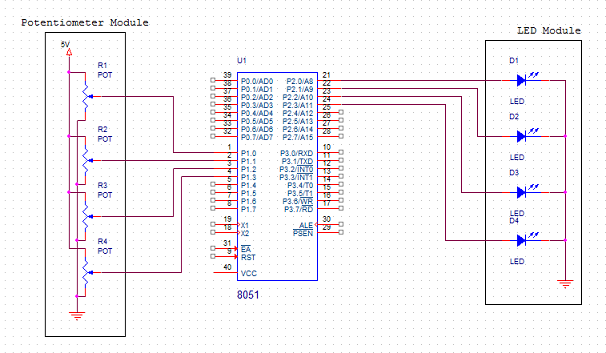
\includegraphics[width=\textwidth]{Schematic.png}
		\caption{Circuit schematic for lab}
		\label{schematic}
	\end{figure}
\subsection{Part 1}
\subsubsection{Code}
	\lstinputlisting{part1_publish.c}
\subsection{Part 2}
\subsubsection{Code}
	\lstinputlisting{part2_publish.c}	
\subsection{Part 3}
\subsubsection{Code}
	\lstinputlisting{part3_publish.c}
\subsection{Enhancement}
\subsubsection{Code}
	\lstinputlisting{encahncement.c}

\section{References} 
\noindent
``MPS Lab 5," in RPI ECSE Department, 2016. [Online]. Available: \url{http://www.rpi.edu/dept/ecse/mps/MPS_Lab_Ex5-Memory.pdf}. Accessed: Nov. 13, 2016.\\
\newline\noindent
``C8051 Manual," in RPI ECSE Department, 1.4 ed., 2005. [Online]. Available: \url{https://www.ecse.rpi.edu/courses/CStudio/Silabs/C8051F12x-13x.pdf}. Accessed: Nov. 13, 2016.


\end{document}